%%%%%%%%%%%%%%%%%%%%%%%%%%%%%% PREAMBLE %%%%%%%%%%%%%%%%%%%%%%%%%%%%%%

\title{Classification of Finitely Often Self-Intersecting Loops in $\mathbb{R}^{2}$ under equivalence given by isomorphism of corresponding Region Graphs.}
\author{
        Adam Kurkiewicz \\
        School of Computer Science \\
        University of Glasgow \\
        United Kingdom \\
}
\date{\today}
\documentclass{article}

\usepackage[british]{babel}

\usepackage{amssymb}
\usepackage{amsthm}
\usepackage{amsmath}
\usepackage{graphicx}
\usepackage{epstopdf}

\theoremstyle{definition}
\newtheorem{definition}{Definition}

\theoremstyle{definition}
\newtheorem{example}{Example}

\theoremstyle{plain}
\newtheorem{proposition}{Proposition}

\newtheorem{theorem}{Theorem}
\begin{document}
\maketitle

%%%%%%%%%%%%%%%%%%%%%%%%%%%%%% FIGURES %%%%%%%%%%%%%%%%%%%%%%%%%%%%%%

\begin{figure}
\centering
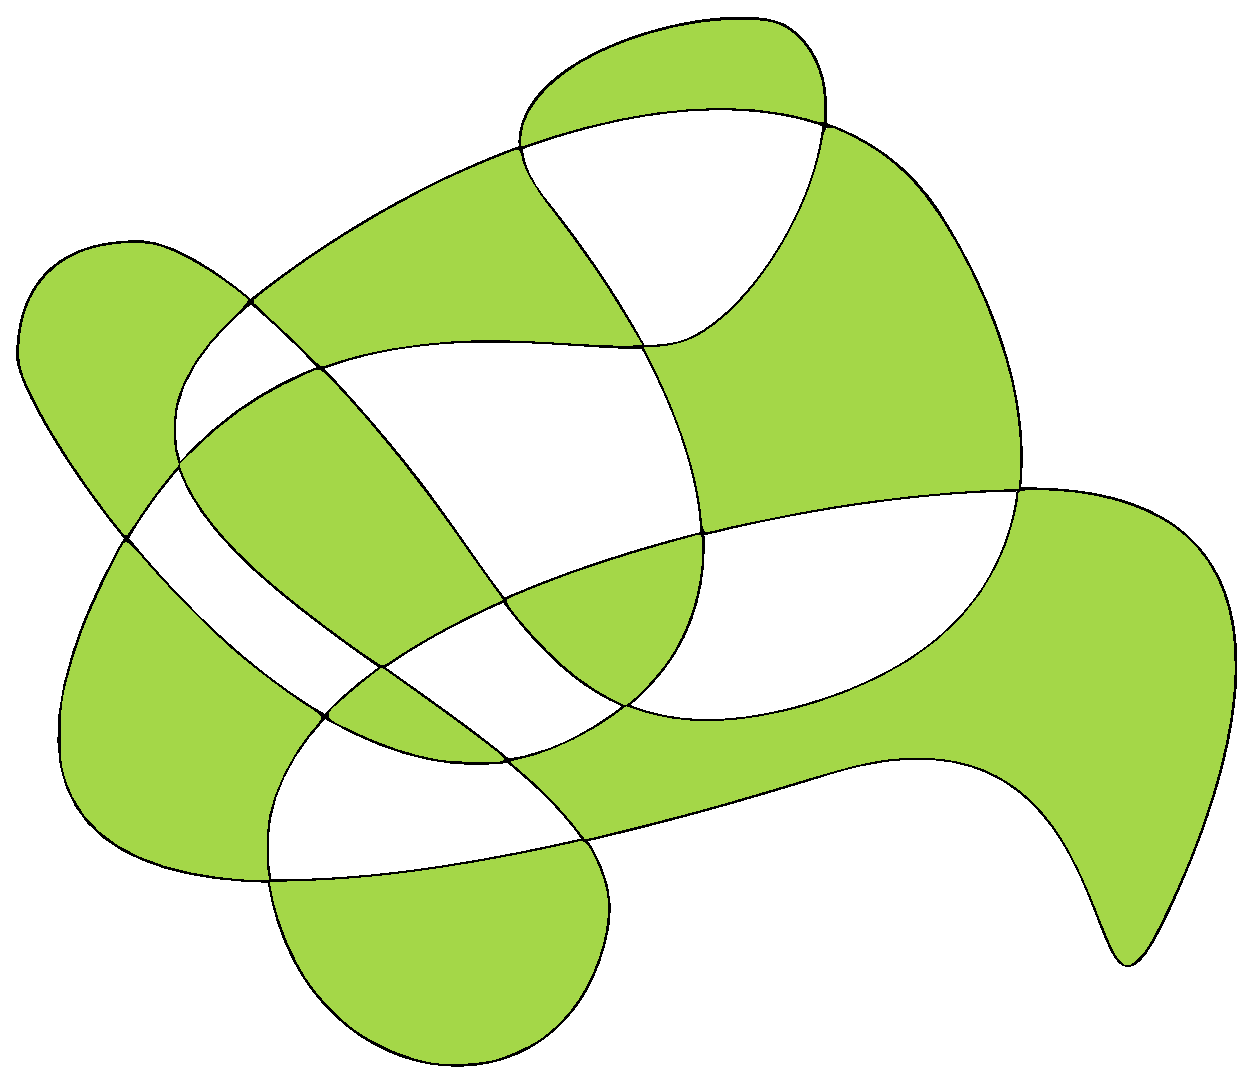
\includegraphics[width=10cm]{curve1.eps}
\caption{2-colouring of a closed loop drawn on a sheet of paper.}
\label{figure:curve1}
\end{figure}

\begin{figure}
\centering

\includegraphics[width=10cm]{curve2.eps}
\caption{Region graph of the closed loop from Figure \ref{figure:curve1}. Vertices corresponding to regions enclosed by the loop are numbered.}
\label{figure:curve2}
\end{figure}

%%%%%%%%%%%%%%%%%%%%%%%%%%%%%% ABSTRACT %%%%%%%%%%%%%%%%%%%%%%%%%%%%%%

\begin{abstract}
Abstract placeholder
\end{abstract}

%%%%%%%%%%%%%%%%%%%%%%%%%%%%%% INTRODUCTION %%%%%%%%%%%%%%%%%%%%%%%%%%%%%%

\section{Introduction}
This work stems from an intuitive observation that for any loop one can draw on a sheet of paper there seems to exist a colouring, which assigns one of two possible colours to any region enclosed by the loop, such that no two neighbouring regions share the same colour. Figure \ref{figure:curve1} gives a graphical representation of this intuition. We can go further and view coloured regions as vertices in a graph, with vertices representing any two neighbouring regions connected with an edge. Figure 2 shows such a graph derived from the loop in Figure \ref{figure:curve1}. It is natural to consider all possible graphs that can be constructed in such way. Can we describe this collection precisely using familiar graph theoretic adjectives (bipartite, planar, connected, etc.)?

%Although graph theory is a child of topology, modern development separated  from its parent developing its own tools and methods. This work, somewhat unusually, takes as much from classical topology (homeomorphism, path-connectedness) as it does from graph theory (planarity, 2-colourability).
In this work we make rigorous and prove the 2-colourability intution suggested by Figure \ref{figure:curve1} for a certain class of loops. We also identify the class of graphs corresponding to this class of loops, by constructing an appropriate surjective function between the two classes.

\begin{definition}[Almost Injectivity]
Let $f: X \mapsto Y$ be a function. Let us say that $f$ is almost injective, if $f(x_{1})=f(x_{2}) \implies x_{1} = x_{2}$ holds for all but finitely many $x_{i}\in X$.
\end{definition}

\begin{example}[Almost Injective Circle]\label{example:AIC}
$f: [0, 1] \mapsto \mathbb{R}^2$ defined by $$f(x) = (\sin(2 \pi x), \cos(2 \pi x))$$ is an almost injective function, which is injective on $(0, 1)$ and fails to be injective on $\{0, 1\}$. Figure \ref{figure:curve1} is a plot of another almost-injective function.
\end{example}

\begin{definition}[Crossing Set]
Let $f: X \mapsto Y$ be an almost injective function. Let the crossing set $C_{f}$ of $f$ be defined by $$C_{f} = \{x_{1}, x_{2} \mid f(x_{1}) = f(x_{2}) \land x_{1} \neq x_{2}\}$$
\end{definition}

\begin{example}
The set $\{0, 1\}$ is a crossing set of the almost injective circle from Example \ref{example:AIC}.
\end{example}

\begin{definition}[Crossing Equivalence]
Let $C_{f}$ be the crossing set of of an almost injective function $f$. Let crossing equivalence $\sim_{C}$ be a relation on $C_{f}$ defined by $c_{1} \sim_{C} c_{2} \iff f(c_{1})=f(c_{2})$ for any $c_{1}, c_{2} \in C_{f}$.
\end{definition}

\begin{proposition}[Crossing Equivalence Relation]
Crossing equivalence $\sim_{C}$ is an equivalence relation on the crossing set $C_{f}$ of an almost injective function $f$.
\end{proposition}

\begin{proof}
Reflexivity, Symmetry and Transitivity follow easily from properties of set equality $=$, and that $f$ is a function.
\end{proof}

\begin{definition}[FOSIL]
Let $\gamma : [0, 1] \mapsto \mathbb{R}^{2}$ be a continuous, almost injective function with $\gamma(0) = \gamma(1)$. We will say that $\gamma$ is a finitely often self-intersecting loop in $\mathbb{R}^{2}$, or FOSIL in short.
\end{definition}

\begin{definition}[Region Number]
Let $\gamma$ be a FOSIL. Let $\sim_{C}$ be a crossing equivalence on $C_{\gamma}$, the crossing set of $\gamma$. Define region number of $\gamma$, $\rho_{\gamma}$ as $$\rho_{\gamma} = 1 + \sum_{[c]\in C_{\gamma}/\sim_{C}}{(\lvert[c]\rvert - 1)}$$.
\end{definition}

\begin{definition}[Regions]
Let $\gamma$ be a FOSIL. Let $R^{\gamma}$ denote a collection of open, connected, disjoint subsets of $\mathbb{R}^{2}$, whose union gives the complement of $\gamma$, that is $\mathbb{R}^{2}\setminus\gamma([0,1])$. Then $R^{\gamma}$ is called a collection of regions of $\gamma$, and $R_{i} \in R^{\gamma}$ is called a region.
\end{definition}

\begin{theorem}[Jordan Curve Theorem for FOSILs]
Let $\gamma$ be a FOSIL, $R^{\gamma}$ be a collection of regions of $\gamma$, and $\rho_{\gamma}$ be the region number of $\gamma$. Then the collection of regions is unique, and $$\lvert R^{\gamma}\rvert = \rho_{\gamma}$$
\end{theorem}

This auxiliary result has a rather technical proof, to which we devote a separate chapter.

\begin{definition}[Edge-Connectedness]
Let $\gamma$ be a FOSIL. Let $R_{1}, R_{2} \in R^{\gamma}$ be regions of $\gamma$, and $C_{\gamma}$ be the crossing set of $\gamma$. We will say that $R_{1}$ and $R_{2}$ are edge-connected if $R_{1} \neq R_{2}$ and there exists an open, connected subset of $[0, 1]$, say $S$, such that $S \cap C_{f} = \emptyset$, and such that $R_{1} \cup \gamma(S) \cup R_{2}$ is connected.
\end{definition}

\begin{proposition}[Edge-Connectedness Reflexivity]
Edge connectedness on the collection of regions of $\gamma$ is a reflexive relation.
\end{proposition}

\begin{proof}
Reflexivity follows from commutativity of set union $\cup$.
\end{proof}

\begin{definition}[Graph]
Let $V$ be a finite set. Let $E$ be a subset of $V\times V$. Then $G=(V, E)$ is called a graph if for any $(v_{1}, v_{2}) \in E$ we have that $(v_{2}, v_{1}) \in E$. $v \in V$ is called a vertex in G, and $(v_{1}, v_{2}) \in E$ is called an edge in G.
\end{definition}

\begin{definition}[Region Graph]
Let $R^{\gamma}$ be the collection of regions of a FOSIL $\gamma$. Let $E = \{(R_{1}, R_{2}) \in R^{\gamma} \times R^{\gamma} \mid R_{1} \operatorname{edge-connected} R_{2}\}$. Then $G_{\gamma}=(R^{\gamma},E)$ is called a region graph of a FOSIL $\gamma$.
\end{definition}

\begin{proposition}[Region Graph is a Graph]
The region graph $G_{\gamma} = (V, E)$ of a FOSIL $\gamma$ is a graph.
\end{proposition}

\begin{proof}
By Jordan Curve Theorem for FOSILs, $V$ is uniquely defined and finite. Let $(R_{1}, R_{2}) \in E$. Then $(R_{2}, R_{1}) \in E$ by reflexivity of edge-connectedness.
\end{proof}

\begin{definition}[Graph Isomorphism]
Let $G_{1}=(V_{1}, E_{1})$ and $G_{2}=(V_{2}, E_{2})$ be graphs with $\lvert V_{1} \rvert$ = $\lvert V_{2} \rvert$ and $\lvert E_{1} \rvert$ = $\lvert E_{2} \rvert$. We will say that $G_{1}$ is graph isomorphic, $\sim_{G}$, to $G_{2}$ if there exists an injective function $\psi : V_{1} \mapsto V_{2}$ such that for each $(v_{1}, v_{2}) \in E_{1}$, we have that $(\psi(v_{1}), \psi(v_{2})) \in E_{2}$.
\end{definition}

\begin{proposition}[Graph Isomorphism Equivalence Relation]
Let $\mathfrak{G}$ be a collection of graphs. Then $\sim_{G}$ is an equivalence relation on $\mathfrak{G}$.
\end{proposition}
\begin{proof}
TODO Symmetry, transitivity, reflexivity.
\end{proof}

\begin{definition}[Path in Graph]
Let $G=(V, E)$ be a graph. Let $P=\{v_{k}\}$ be a sequence of vertices in G, such that for any $v_{i}, v_{i+1} \in P$, we have that $(v_{i}, v_{i+1}) \in E$. Then $P$ is called a path in graph G.
\end{definition}

\begin{definition}[Connected Graph]
Let $G=(V, E)$ be a graph. Let us say that $G$ is connected if there exists a path $P$ in $G$, such that for any $v \in V$ we have that $v \in P$.
\end{definition}

\begin{definition}[Bipartite Graph]
Let $G=(V,E)$ be a graph. If there exist disjoint $S_{1}, S_{2} \subseteq V$ with $S_{1} \cup S_{2} = V$ such that for any $v_{i}, w_{i} \in S_{i}$ we have $(v_{i}, w_{i}) \notin E$, then G is called a bipartite graph.
\end{definition}

\begin{definition}[Planar Graph]
TODO define planar graphs.
\end{definition}

\begin{theorem}[FOSIL Classification Theorem]

Let $\mathfrak{F}$ be the collection of all FOSILs. Let $\mathfrak{G}=\{G_{\gamma} | \gamma \in \mathfrak{F}\}$ be the collection of corresponding region graphs. Let $\mathfrak{B}$ be the collection of all connected, bipartite, planar graphs, containing more than 1 vertex. By abuse of notation, let $\sim_{G}$ denote the equivalence relation given by graph isomorphism on both $\mathfrak{G}$ and $\mathfrak{B}$. The function $$\Phi : \mathfrak{G}/\sim_{G} \mapsto \mathfrak{F}/\sim_{G}$$ given by $$\Phi([G]_{\mathfrak{G}}) = [G]_{\mathfrak{B}}$$ is a well-defined bijection.

In other words, $\mathfrak{G} \subseteq \mathfrak{B}$ and for any $B \in \mathfrak{B}$ there is a $G \in \mathfrak{G}$ with $G \sim_{G} B$.
\end{theorem}
We devote the next chapter to the proof of this theorem.

\section{FOSIL Classification Theorem}

The inclusion bit should follow from Hopf's degree theorem. Surjectivity is much trickier, but there seems to be an algorithm to go from any bipartite graph to a FOSIL, but I don't quite have the details yet.

\section{Jordan Curve Theorem for FOSILs}

The starting point should be the proof of Jordan-Holder. Two proofs in particular seem of interest \cite{hales07}, \cite{thomassen92}.

\bibliographystyle{abbrv}
\bibliography{kurkiewicz16.bib}

\end{document}
